\chapter{Results and Discussion}\label{chap:results_discussion}
\section{Results}\label{sec:results}
\subsection{Metrics for Binary Classification}\label{sec:confusion_matrix}
When evaluating the effectiveness of a binary prediction technique using a validation dataset with known activities, four central values are considered:

\begin{enumerate}
  \item True Positives (TP): The number of correctly predicted active cases.
  \item True Negatives (TN): The number of correctly predicted inactive cases.
  \item False Positives (FP): The number of incorrectly predicted active cases.
  \item False Negatives (FN): The number of incorrectly predicted inactive cases.
\end{enumerate}

Using these four values, it is possible to construct a confusion matrix and derive evaluation metrics, as illustrated in Figure~\ref{fig:confusion_matrix}:

\begin{figure} 
  \centering
  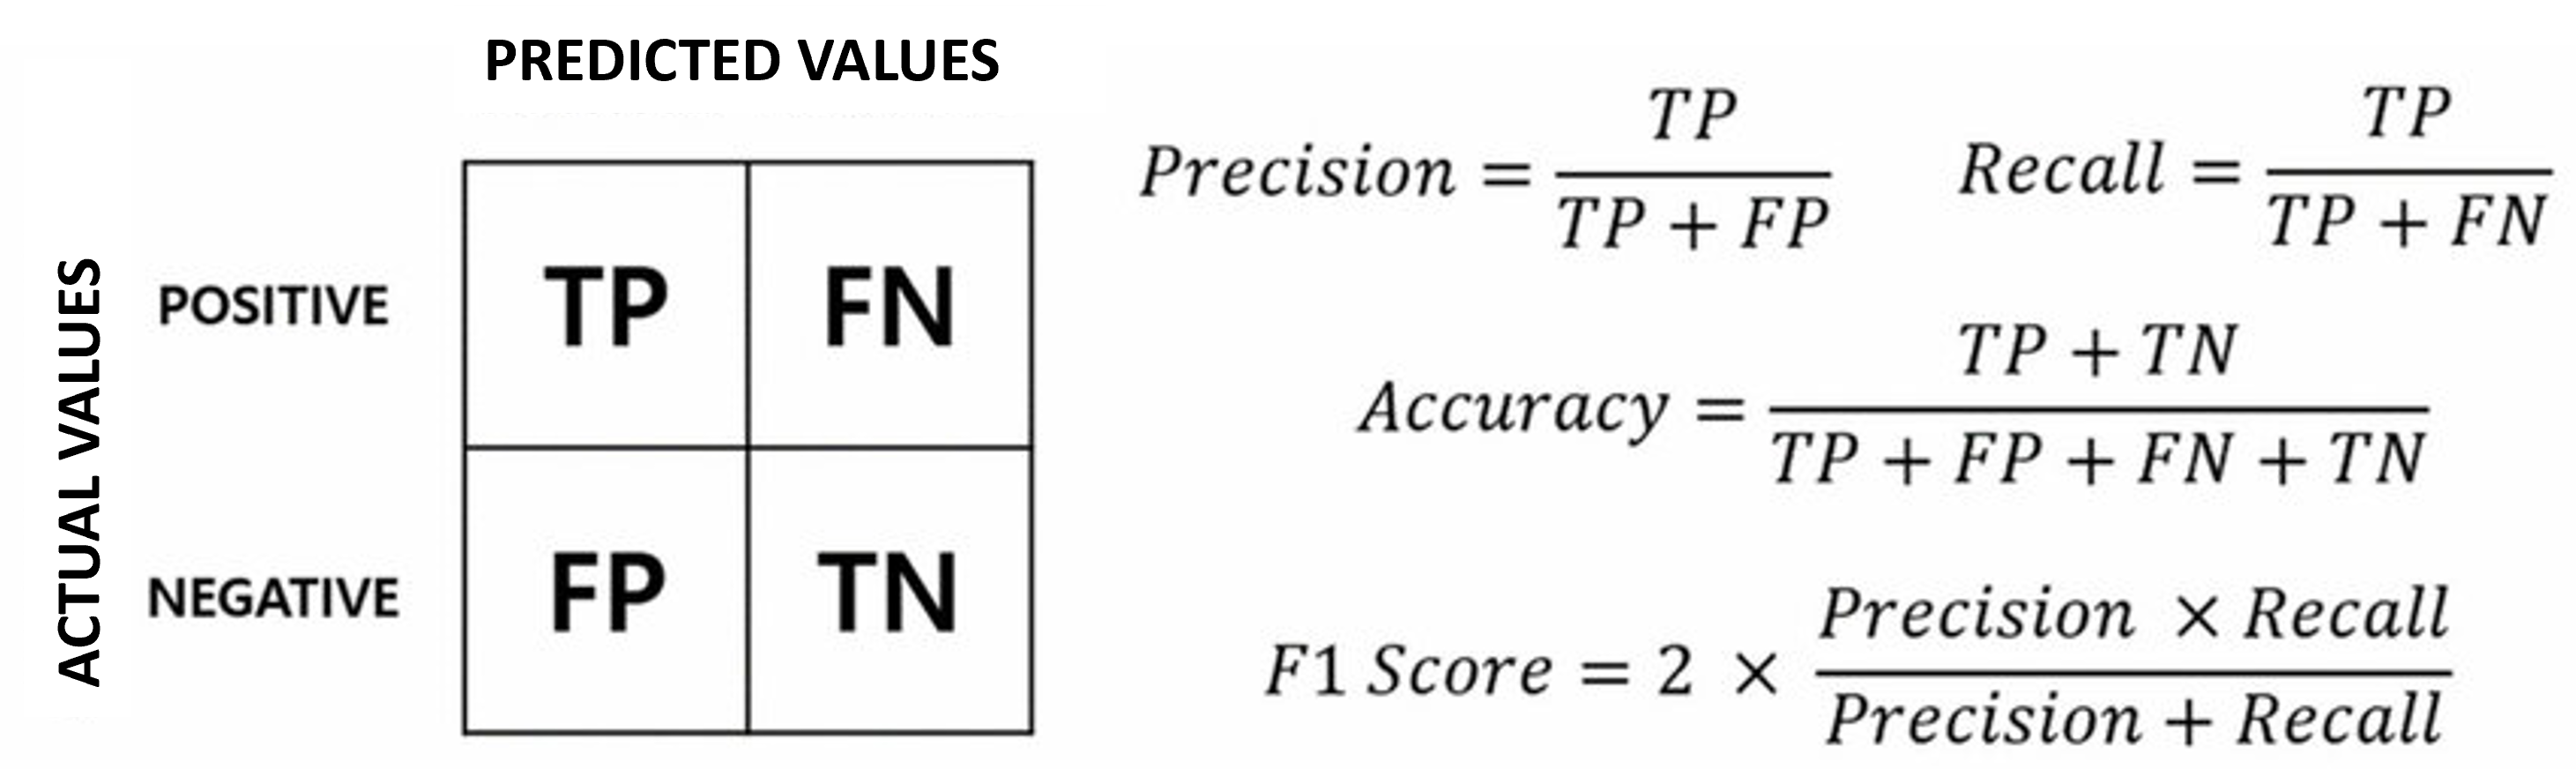
\includegraphics[width=1.0\textwidth]{figures/confusion_matrix_metrics.png}
  \caption{Confusion Matrix and Metrics: Accuracy, Precision, Recall, and F1 score.
  Figure obtained from~\cite{seol2023}.}
~\label{fig:confusion_matrix}
\end{figure}

\begin{figure} 
  \centering
  \includegraphics[width=1.0\textwidth]{figures/roc97.png}
  \caption{For assay endpoint with aeid: 97, the Receiver Operating Characteristic (ROC) curve is shown for the XGBoost Classifier. We predicted each trained model with four different classification thresholds, namely default = 0.5, optimal = cost(TPR, FPR), True Positive Rate = 0.5 (tnr), True Negative Rate = 0.5 (tnr).}
~\label{fig:confusion_matrix}
\end{figure}


\begin{figure} 
  \centering
  \includegraphics[width=1.0\textwidth]{figures/cm97.png}
  \caption{For assay endpoint with aeid: 97, confusion matices are shown for four different classification thresholds.}
~\label{fig:confusion_matrix}
\end{figure}



\subsection{Evaluation}\label{sec:evaluation}
\begin{figure} 
  \centering
  \includegraphics[width=1.0\textwidth]{figures/val.png}
  \caption{Summary of results for internal validation set}
~\label{fig:confusion_matrix}
\end{figure}

\begin{figure} 
  \centering
  \includegraphics[width=1.0\textwidth]{figures/mb_val_structure.png}
  \caption{Summary of results for MassBank validation set with fingerprints derived from chemical structures}
~\label{fig:confusion_matrix}
\end{figure}

\begin{figure} 
  \centering
  \includegraphics[width=1.0\textwidth]{figures/mb_val_sirius.png}
  \caption{Summary of results for MassBank validation set with SIRIUS-predicted fingerprints}
~\label{fig:confusion_matrix}
\end{figure}

\section{Discussion}\label{sec:discussion}


